\documentclass[11pt,professionalfonts]{beamer}
\usefonttheme{serif}

\usepackage{aas_presentation_packages}
\usepackage{tikz_packages}
\tdplotsetmaincoords{60}{125} % view angle in spherical coordinates

\bibliography{library} % must be in the preamble when using biblatex package

\DeclareSIUnit\year{yr}

\newcommand{\vs}{\vspace{0.3cm}}

\definecolor{mygray}{gray}{0.9}
\definecolor{RoyalBlue}{rgb}{0.25,0.41,0.88}
\def\Emph{\textcolor{RoyalBlue}}

\definecolor{tmp}{rgb}{0.804,0.941,1.0}
\setbeamercolor{numerical}{fg=black,bg=tmp}
\setbeamercolor{exact}{fg=black,bg=red}

\mode<presentation> 
{
  \usetheme{Warsaw}
  \usefonttheme{serif}
  \setbeamercovered{transparent}
}

\setbeamertemplate{footline}%{split theme}
{%
  \leavevmode%
  \hbox{\begin{beamercolorbox}[wd=.5\paperwidth,ht=2.5ex,dp=1.125ex,leftskip=.3cm,rightskip=.3cm plus1fill]{author in head/foot}%
    \usebeamerfont{author in head/foot}\insertshorttitle
  \end{beamercolorbox}%
  \begin{beamercolorbox}[wd=.5\paperwidth,ht=2.5ex,dp=1.125ex,leftskip=.3cm,rightskip=.3cm]{title in head/foot}
%    \usebeamerfont{title in head/foot}\mypaper\hfill \insertframenumber/\inserttotalframenumber
    \usebeamerfont{title in head/foot}\hfill \insertframenumber/\inserttotalframenumber
  \end{beamercolorbox}}%
  \vskip0pt%
} \setbeamercolor{box}{fg=black,bg=yellow}


\title[Reachability Sets on a \Poincare section]{\large\bf  Low-Thrust Trajectory Design Using Reachability Sets near Asteroid 4769 Castalia}

\author{\vspace*{-0.3cm}}

   
\institute{
  \footnotesize
  {\normalsize\bf{Shankar Kulumani}}\\
  \vspace*{0.2cm}
    \textbf{Flight Dynamics \& Control Lab}\\ \vspace*{0.5cm}
  \begin{figure} %figure%
        \includegraphics[width=0.75\textwidth]{gw_txh_2cs_pos}
    \end{figure}
}
\date{}

\begin{document}
%=======================================================%

\setcounter{framenumber}{-1}
\begin{frame} %-----------------------------%
  \titlepage
\end{frame}   %-----------------------------%

\section*{}
\subsection*{Introduction}  

\begin{frame}{Asteroid Missions}
\begin{itemize}
    \item Science - insight into the early formation of the solar system
    \item Mining - vast quantities of useful materials
    \item Impact - high risk from hazardous near-Earth asteroids
\end{itemize}    

\begin{center}
    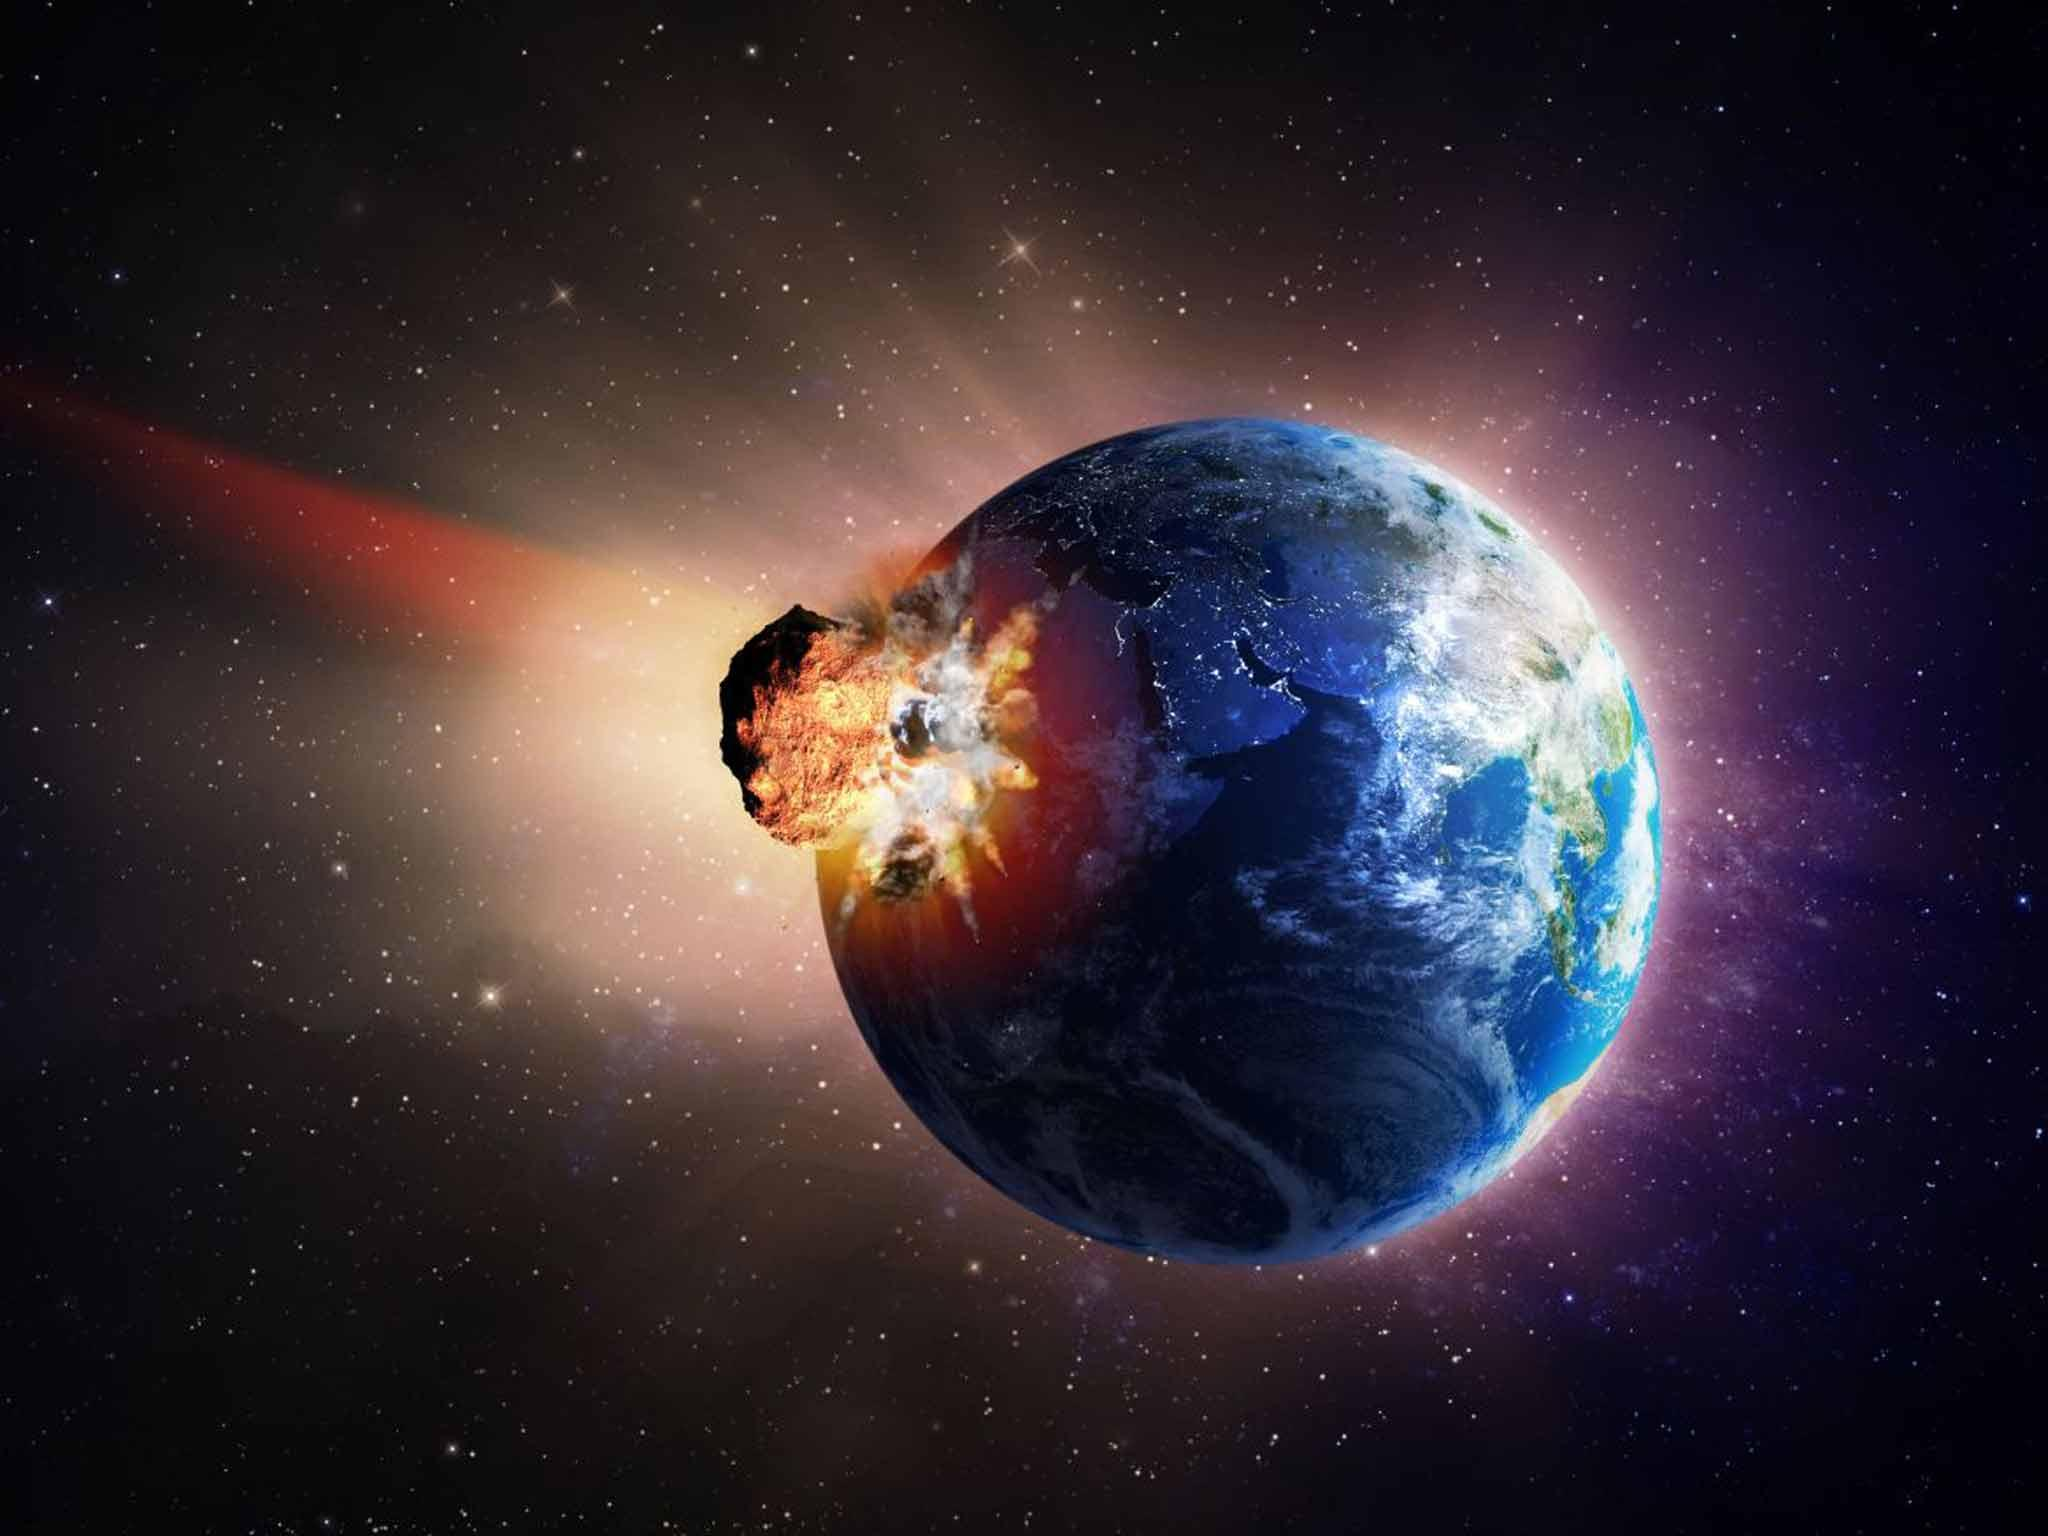
\includegraphics[height=0.35\textheight]{figures/asteroid-alamy.jpg}
    \hfill
    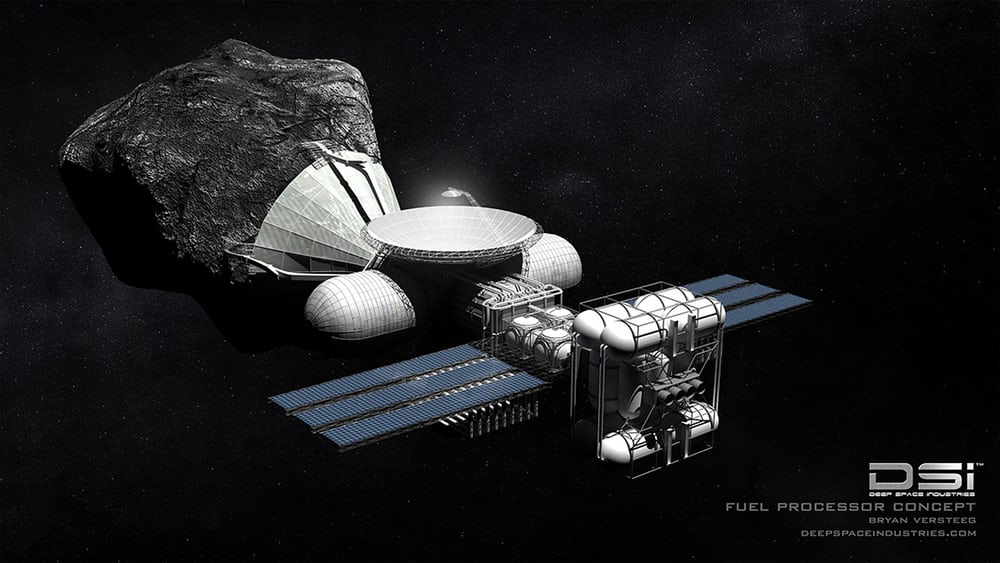
\includegraphics[height=0.35\textheight]{figures/asteroid-mining-feature-8.jpg}
\end{center}
\end{frame}

\begin{frame}{Asteroid Mining}
    \begin{itemize}
      \item Useful materials can be extracted from asteroids to support:
      \begin{itemize}
          \item Propulsion, construction, life support, agriculture, and precious/strategic metals
      \end{itemize}
      \item Commercialization of near-Earth asteroids is feasible~\footfullcite{ross2001}
    \end{itemize}

\pause

\begin{center}
\small
    \begin{tabular}{|l|r|r|}
        \hline 
        Element & Price (\SI{}{\$\per\kilo\gram}) & Sales (\SI{}{\$M\per\year}) \\
        \hline \hline 
        Phosphorous (P) & \num{0.08}  & \num{2167} \\
        Gallium (Ga) & \num{300.00}  & \num{1544} \\
        Germanium (Ge) & \num{745.00} & \num{6145} \\
        \hline \hline 
        Platinum (Pt) & \num{12394.00} & \num{1705} \\
        Gold (Au) & \num{12346.00} & \num{49} \\
        Osmium (Os) & \num{12860.00} & \num{307} \\
        \hline
    \end{tabular}
\end{center}

\end{frame}


\section*{}
\subsection*{System Model}

\begin{frame}{Gravitational Modeling} %-----------------------------%

\begin{itemize}
    \item Potential is a function of only the shape model
    \item Globally valid, closed-form expression of potential
    \item Exact potential assumes a constant density 
    \item Accuracy solely dependent on shape model
\end{itemize}
\only<2>{
\begin{align*}\label{eq:potential}
    U(\vecbf{r}) &= \frac{1}{2} G \sigma \sum_{e \in \text{edges}} \vecbf{r}_e \cdot \vecbf{E}_e \cdot \vecbf{r}_e \cdot L_e - \frac{1}{2}G \sigma \sum_{f \in \text{faces}} \vecbf{r}_f \cdot \vecbf{F}_f \cdot \vecbf{r}_f \cdot \omega_f 
\end{align*}
}
\only<3>{
\begin{center}
  \animategraphics[autoplay,loop,width=0.5\textwidth]{30}{./animation/castalia/IMG}{00001}{00999}~\hfill
  \includegraphics[width=0.5\textwidth]{figures/radius_contour.pdf}
\end{center}
}

\end{frame}

\begin{frame}{Equations of Motion}

\begin{itemize}
    \item Many similarities to the three-body problem
    \item Equations are also defined in rotating frame
\end{itemize}

\[
    \begin{bmatrix} \dot{\vecbf{r}} \\ \dot{\vecbf{v}} \end{bmatrix} =
    \begin{bmatrix}\vecbf{v} \\ \vecbf{g} \parenth{\vecbf{r}} + \vecbf{h}\parenth{\vecbf{v}} + \vecbf{u} \end{bmatrix} 
\]
\pause
\begin{itemize}
    \item Dynamics allow for a single integral of motion 
    \item Differential correction used to find periodic orbits
\end{itemize}

\[
    J \parenth{\vecbf{r}, \vecbf{v}} = \frac{1}{2} \omega^2 \parenth{x^2 + y^2} + U(\vecbf{r}) - \frac{1}{2} \parenth{\dot{x}^2 + \dot{y}^2 + \dot{z}^2} 
\]
\end{frame}

\section*{}
\subsection*{Technical Approach}

\begin{frame}{Proposed Approach} % -----------------------------------%
  \begin{itemize}
      \item \Emph{Reachability set} on \Poincare section allows for systematic transfer design
        \begin{itemize}
            \item Transfer design on lower dimensional subspace
            \item Simple method to incorporate effects of low-thrust 
            \item Avoids the issue of determining initial conditions
        \end{itemize}
        \pause
      \item Extension of previous work in planar three-body problem     
  \end{itemize}

  \note[itemize]{
    \item Reachability set avoids the need to pick initial conditions
    \item We compute on a lower dimensional surface
  }
\end{frame} %--------------------------------------%

\begin{frame}{Reachability Sets and the \Poincare map}
\begin{itemize}
    \item Intersections of trajectories with a lower dimensional surface
        \pause
        \begin{itemize}
            \item The \Poincare section, \( \Sigma \), reduces the computational complexity 
            \item Useful for investigating the stability and structure of the system
        \begin{align*}
            \Sigma = \braces{\parenth{x, \dot{x}, z, \dot{z}} | y(t_f) = 0 }
        \end{align*}
        \end{itemize}
        \pause
    \pause
    \item \Poincare section serves as subspace for the reachability set
    \begin{itemize}
        \item Set of states achievable from a given initial condition over fixed \( t_f \) s.t. maximum control constraint
        \begin{align*}
            R( \vecbf{x}_0, \mathcal{U} , t_f) = \braces{ \vecbf{x}_f \subseteq \mathcal{X} | \exists \vecbf{u} \in \mathcal{U}, \vecbf{x}(t_f) = \vecbf{x}_f }
        \end{align*}
        \pause
        \item Directly derivable from optimal control
        \item Frequently used for safety planning, e.g. air traffic avoidance
        \pause
        \item We extend its use to the design of spacecraft transfers
    \end{itemize}
\end{itemize}

\end{frame}

\begin{frame}{Reachability Set on \Poincare section} % -----------------------------------%

\begin{itemize}
    \item Generate the reachability set on a \Poincare section
    \[
        \Sigma = \braces{\parenth{x, \dot{x}, z, \dot{z}} | y(t_f) = 0 }
    \]
    \item Control input is chosen to enlarge the reachable set
\end{itemize}
\pause
\begin{figure}
    \centering
    \begin{scaletikzpicturetowidth}{0.7\textheight}
    \begin{tikzpicture}[tdplot_main_coords,
          poincare/.style={opacity=.2,very thick,fill=blue},
          orbit/.style={very thick,black},
          orbit hidden/.style={very thick,dashed},
          grid/.style={very thin,black},
          axis/.style={->,blue,thick},
          reachability/.style={thick,blue}, scale=\tikzscale]

        \pause
        % nodes for the poincare section
        \node[label=above:\(\Sigma\)] (upper_right) at (0,5,5) {};
        \node[] (upper_left) at (0,1,5) {};
        \node[] (lower_left) at (0,1,0) {};
        \node[] (lower_right) at (0,5,0) {};
        
        % draw poincare section
        \draw[poincare] (upper_right.center) -- (upper_left.center) -- (lower_left.center) -- (lower_right.center) -- (upper_right.center);
       
        \pause
        % draw a periodic orbit
        \coordinate (center) at (0,0,2);
        \node[label=below:\(\vecbf{x}_0\)] (x0) at (0,3,2) {};
        % \node[label=below:\(\vecbf{x}_n\)] at (x0) {};
        \filldraw (x0) circle (3pt);

        % \tdplotdrawarc[orbit hidden]{(center)}{3}{90}{200}{}{};
        \tdplotdrawarc[orbit,<-]{(center)}{3}{-160}{90}{}{};
        \pause
        % draw reachability set on the poincare section
        \coordinate (reach) at (0,4.5,2);
        \tdplotsetthetaplanecoords{90}

        \draw[tdplot_rotated_coords,grid] (x0) -- (reach);
        \draw[tdplot_rotated_coords,grid] (x0) -- ++(-45:1.5);

        \tdplotdrawarc[tdplot_rotated_coords,grid]{(x0)}{0.5}{-45}{90}{above}{\(\phi\)};
        \pause
        % draw terminal state on reachability set
        \node[tdplot_rotated_coords,label=above:\(\vecbf{x}_f\)] (xf) at ($ (x0)+(-45:1.5) $) {};
        \filldraw (xf) circle (3pt);

        \node[tdplot_rotated_coords,label=below:\(J\)] at (xf) {};

        \tdplotdrawarc[tdplot_rotated_coords,reachability]{(x0)}{1.5}{0}{360}{}{};
        % place
    \end{tikzpicture}
    \end{scaletikzpicturetowidth}
\end{figure}

\end{frame} %--------------------------------------%

\begin{frame}{Optimal Control Problem}
\begin{itemize}
    \item Reachability defined as distance between controlled and uncontrolled states
    {\small
        \[
            J = -\frac{1}{2} \left( \vecbf{x}(t_f) - \vecbf{x}_{n}(t_f)\right)^T 
            Q
            \left( \vecbf{x}(t_f) - \vecbf{x}_{n}(t_f)\right) 
        \]
    }
    \pause
    \item Terminal constraints used to ensure correct section and specific direction on \( \Sigma \in \R^4 \)
    {\small
        \begin{align*}\label{eq:terminal_constraints}
            \begin{split}
                m_1 &= y = 0  \\
                m_2 &= \parenth{\sin \phi_{1_{d}}} \parenth{ x_1^2 + x_2^2 + x_3^2 + x_4^2} - x_1^2 = 0 \\
                m_3 &= \parenth{\sin \phi_{2_{d}}} \parenth{ x_2^2 + x_3^2 + x_4^2} - x_2^2 = 0\\
                m_4 &= \parenth{\sin \phi_{3_{d}}} \parenth{ 2 x_3^2 + 2 x_3 \sqrt{x_4^2 + 2 x_4^2}} - x_3 - \sqrt{x_4^2 + x_3^2} = 0 
            \end{split}
        \end{align*}
    }
    \pause
    \item Control constraint used to emulate realistic system
        {\small
        \[
            c(\vecbf{u}) = \vecbf{u}^T \vecbf{u} - u_m^2 \leq 0 
        \]
        }
\end{itemize}

\end{frame}

\section*{}
\subsection*{Numerical Simulation}

\begin{frame}{Transfer Objective} %-----------------------------%

\begin{itemize}
    \item Goal is to transfer between two equatorial periodic orbits
    \item Typical scenario during study of an asteroid
\end{itemize}

\begin{center}
    \includegraphics[width=0.5\textwidth]{figures/initial_transfer.pdf}
    \hfill
    \includegraphics[width=0.5\textwidth]{figures/initial_transfer_3d.pdf}
\end{center}

\end{frame}%-----------------------------%

\begin{frame}{Simulation}


\begin{itemize}
    \item Generate the reachability set through discretization of \( \phi_i \)
    \item Visualize \( \Sigma \in \R^4 \) through the use of two 2-D sections
    \pause
    \item Control input allows for large deviation in velocity components
\end{itemize}

\begin{center}
    \includegraphics[width=0.5\textwidth]{figures/poincare_xvsxdot.pdf}
    \hfill
    \includegraphics[width=0.5\textwidth]{figures/poincare_zvszdot.pdf}
\end{center}

\end{frame}

\begin{frame}{Simulation}
    \begin{itemize}
        \item Four iterations of the reachable state to meet the target set
        \item Final transfer is computed with a fixed terminal state constraint
    \end{itemize}

    \begin{center}
        \includegraphics[width=0.5\textwidth]{figures/trajectory.pdf}
        \hfill
        \includegraphics[width=0.5\textwidth]{figures/trajectory_3d.pdf}
    \end{center}

\end{frame}

\begin{frame}{Complete transfer}
\begin{itemize}
    \item We can visualize the complete trajectory in both the body and inertial frames
\end{itemize}

\begin{center}
  \animategraphics[autoplay,loop,width=0.5\textwidth]{30}{./animation/body/IMG}{00001}{01499}~\hfill
  \animategraphics[autoplay,loop,width=0.5\textwidth]{30}{./animation/inertial/IMG}{00001}{01499}
\end{center}

\end{frame}

\section*{}
\subsection*{}

\begin{frame}[noframenumbering]{Conclusions} %-----------------------------%
\begin{itemize}
    \item Transfer using multiple iterations of the reachability set
    \item Alleviates the need for selecting accurate initial guesses 
    \item Gives insight into the possible motion of the spacecraft
    \item Extension of work in the planar three-body problem
    \item Future research goals
        \begin{itemize}
            \item Apply Computational Geometric Optimal Control
            \item Lyapunov based feedback control for orbital transfers
        \end{itemize}
\end{itemize}

\end{frame}   %-----------------------------%

\begin{frame}[noframenumbering,c]{Thank you}
  \centering
  
  \textbf{\large Flight Dynamics \& Control Lab} \\
  Mechanical \& Aerospace Engineering \\
  School of Engineering \& Applied Science
  
  \begin{figure} %figure%
        \includegraphics[width=0.75\textwidth]{gw_txh_2cs_pos}
    \end{figure}
  
  \url{https://fdcl.seas.gwu.edu}
\end{frame}

\end{document}

